\documentclass[11pt]{article}
\usepackage{graphicx}

\begin{document}
	
	\begin{center}
		Assignment No 2
	\end{center}•
	
	\noindent
	Aim:\\Implement Recursive Descent Parser for some language.\\
	
	\noindent
	Software:\\
	\begin{enumerate}
		\item Linux Operating System
		\item GCCcompiler
	\end{enumerate}•
	
	\noindent
	MATHEMATICALMODEL:\\
	
	\noindent
	S={s,e,i,o,f,DD,NDD,success,failure}\\
	s=Start of program\\
	e=The end of program\\
	i=Input String to be parsed. o=Output of the parser, ie, \\
	ValidString(if given input string is valid) OR Parse error (if given input string is invalid)\\
	Success-Parser gives expected output\\
	Failure-Power Failure, Insufficient Memory. f={E, Eprime, T, Tprime, F}\\
	
	\noindent
	Theory:
	
	\noindent
	Recursive Descent Parser\\
	
	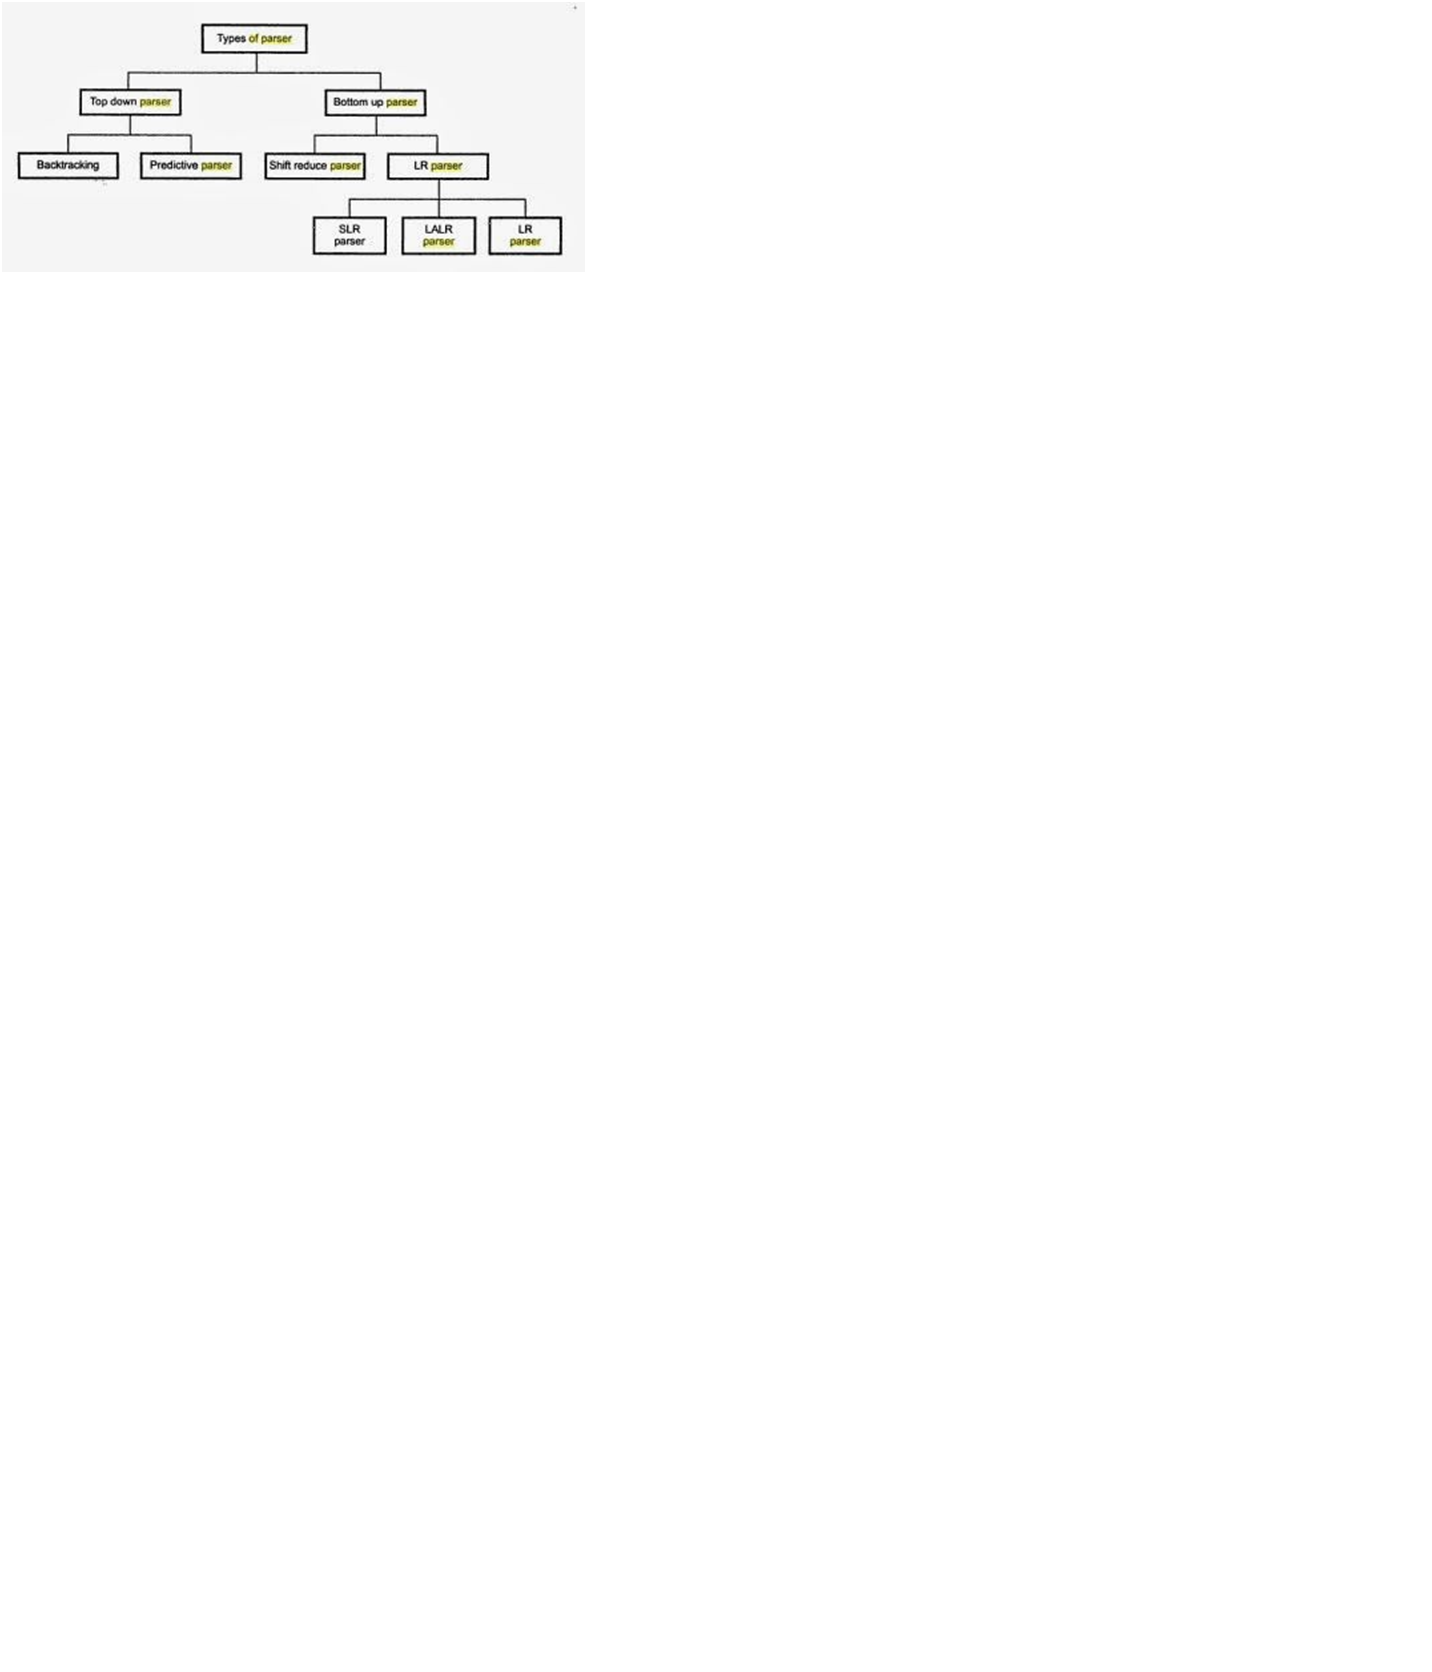
\includegraphics{image1.png}
	
	\noindent
	This is a top-down parser in which the parser attempts to verify that the syntax of the input stream is correct as it is read from left to right. A basic operation necessary for this  involves reading characters from the input stream and matching then with terminals from the grammar that describes the syntax of the input.RDP will look ahead one character and advance the input stream reading pointer when proper matches occur.\\
	
	RDP consists of a set of procedures, one for each non terminal. Execution begins with the procedure of the start symbol, which halts and announces success if its procedure body scans the entire input string (valid).\\
	
	RDP may require back tracking; that is, it may require repeated scans over the input. Parse tree with all possible alternatives. If one alternative doesn’t workout, backtrack and use another alternative. If even after using allalternatives, required string is not formed, string is invalid.Consider the following grammar.The required string is ”cad”:\\
	
	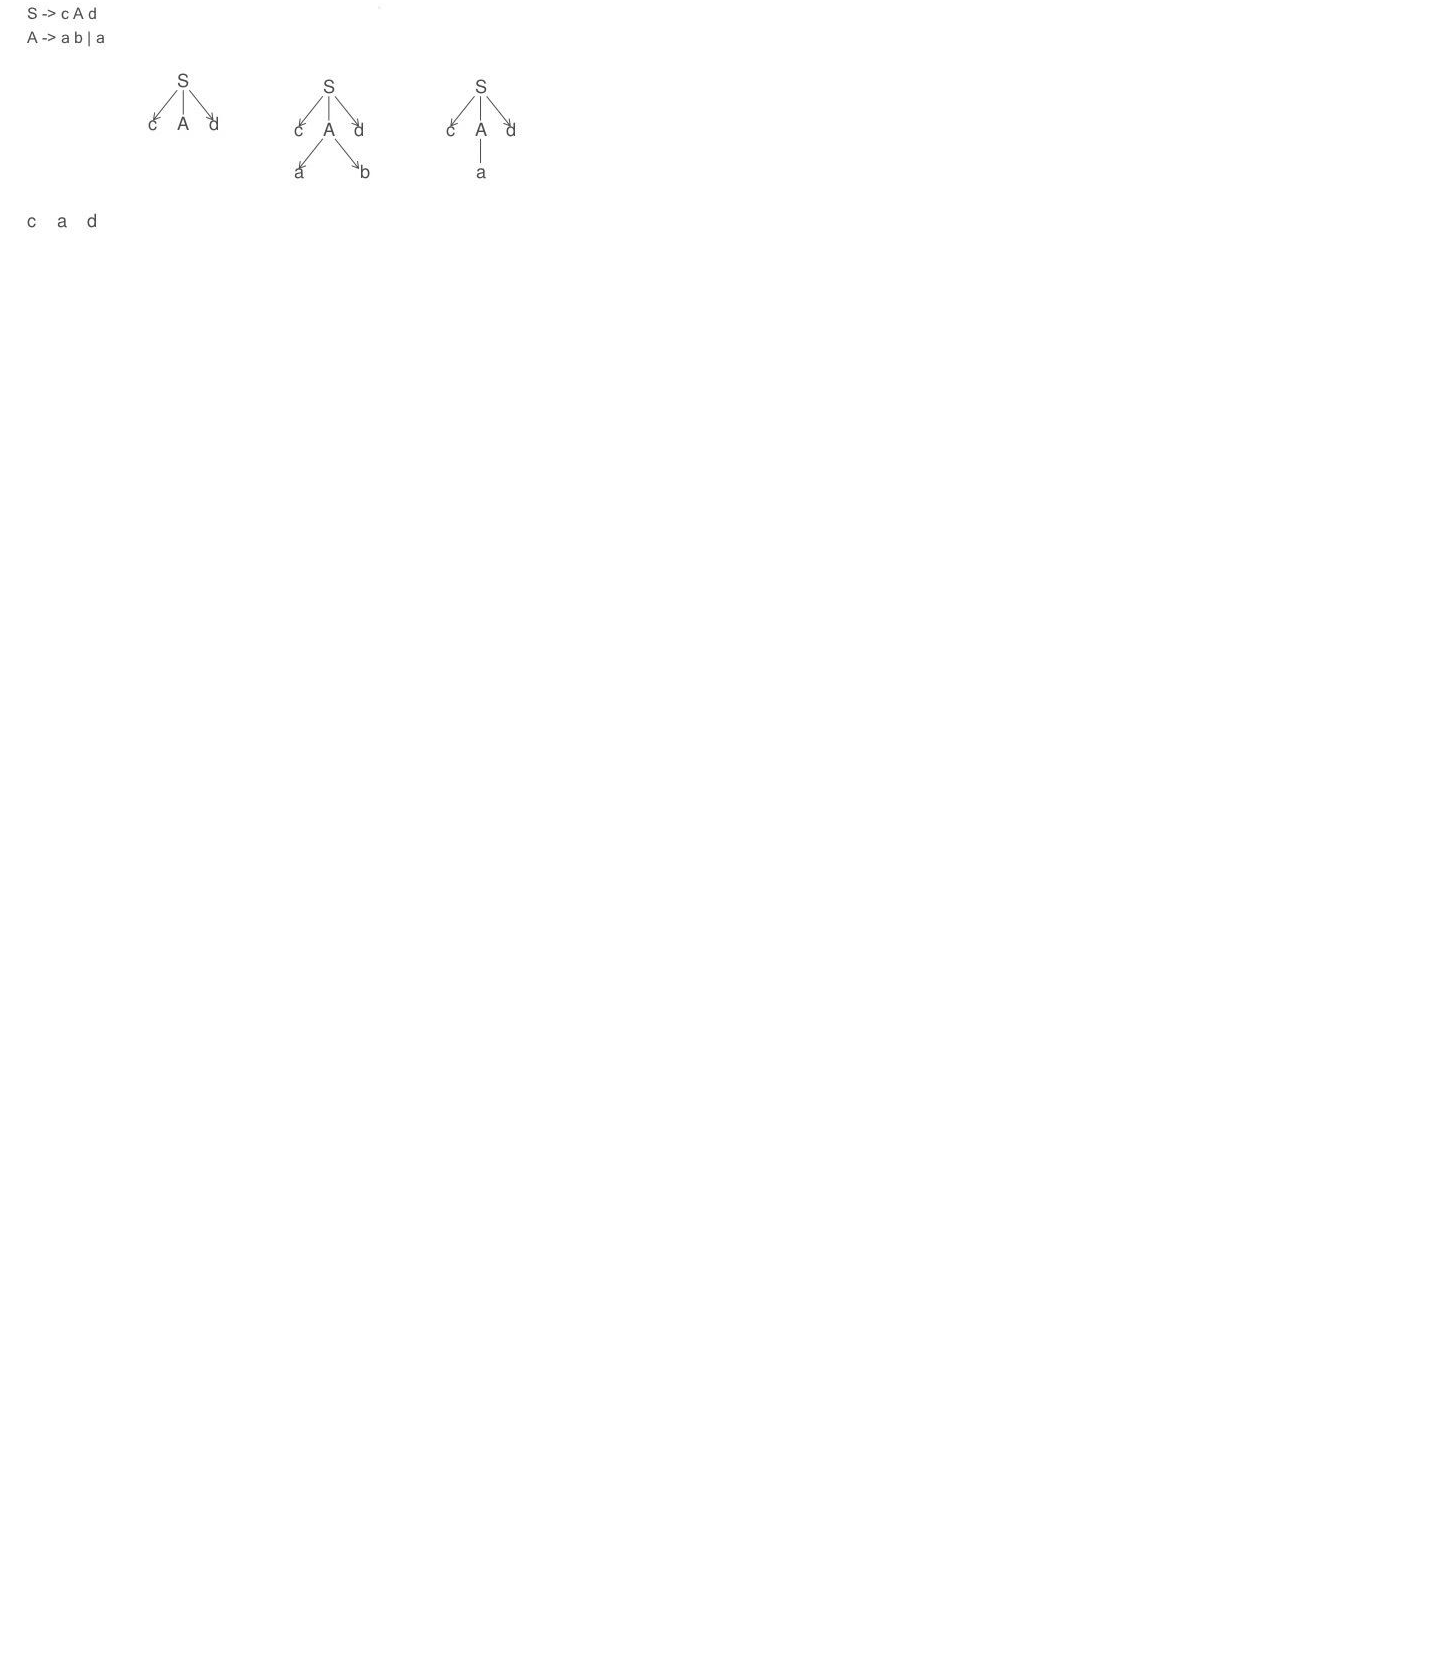
\includegraphics{image2.png}
	
	\noindent
	Advantage:\\
	1.Construction of RDP is easy.\\
	
	\noindent
	Disadvantages:\\
	1.Backtracking(Not allowed in many programming languages)\\
	2.For left recursive grammar RDP parser may fall in infinite loop.\\
	3.Large space to be traversed (multi level backtracking as parse tree is derived blindly)\\
	
	\noindent
	Construction of Recursive Descent Parser:\\
	\begin{enumerate}
		\item If input symbol is non terminal then a call to the procedure correspond-ing to the non terminal is made.
		\item If input symbol is terminal then it is matched with the look ahead from input. The look ahead pointer has to be advanced on matching of the input symbol.
		\item If the production rule has many alternates then all these alternates has to be combined into a single body of procedure.
		\item The parser should be activated by a procedure corresponding to the start symbol.
		
	\end{enumerate}•
	
	\noindent
	Command:\\
	\$gccRDescent.c\\
	\$./a.out\\
	
	\noindent
	CONCLUSION:\\
	Thus we have constructed Recursive Descent Parser for given grammar.\\
	
	\begin{center}
		\begin{tabular}{|c|c|c|c|c|}
			•$Roll$ $No$ & $Name$ $of$ $Student$ & $Date$ $of$ $performance$ & $Date$ $of$ $Checking$ & $Signature$ $of$ $Staff$ \\ \hline
			•$BECOC357$ & Sunny Shah& 07 / 07 / 2017& 07 / 07 / 2017 &  \\ \hline
		\end{tabular}•
	\end{center}•
	
	\newpage
	\section{PLAGARISM REPORT :}
	\begin{figure}[h!]
		\centering
		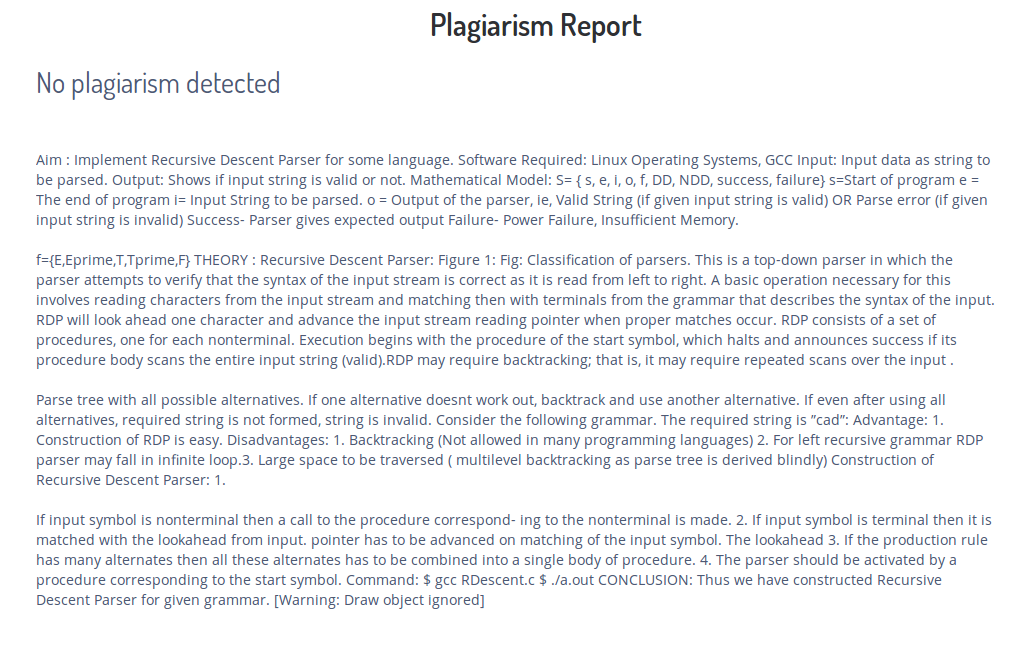
\includegraphics[height=4in,width=4in]{plagiarism2.png}
		\caption{Plagarism Checker www.smallseotools.com/plagarism-checker}
	\end{figure}
	\newpage
\end{document}

